<<<<<<< 748b67fd60b26d45750e10209255345ebe612814
\section{Theorie}
\label{sec:Theorie}

%\cite{sample}
||||||| merged common ancestors
\section{Theorie}
\label{sec:Theorie}

%\cite{sample}
=======
\section{Theorie}
\subsection{Köhärenz und Interferenz von Licht}
Licht ist eine Elektromagnetische Welle und lässt sich durch die Maxwellgleichungen
beschreiben. Der einfachste Fall einer Welle ist die ebene Welle, deren elektrisches Feld
wie folgt dargestellt werden kann:
\begin{equation}
  \vec{E}(x,t)=\vec{E}_{0}\cos(kx-\omega t -\delta)
  \label{eqn:eben}.
\end{equation}
Dabei bezeichnet $k=\frac{2\pi}{\lambda}$ die Wellenzahl mit der Wällenlänge $\lambda$,
$\omega$ ist die Kreisfrequenz und $\delta$ bezeichnet eine Phasenverschiebung.
Da es sich bei den Maxwellgleichungen um lineare Differentialgleichungen handelt
gilt das Superpositionsprinzip. Treffen also mehrere Wellen in einem Punkt P
aufeinander überlagern sich die einzelnen Wellen.\\
Die elektrische Feldstäre kann aufgrung ihrer hohen Frequenz %(ca. $\SI{10^{15}}{\Hz}$)
nicht direkt gemessen werden. Daher wird folgende Gleichung ausgenutzt

\begin{equation}
  I=\text{const} |\vec{E}|^{2}
  \label{eqn:intensität}
\end{equation}

und statt des elektrischen Feldes wird die Intensität bestimmt.
\label{sec:Theorie}
Mit Hilfe dieser Gleichung lässt sich eine Formel für die Intensität zweier
überlagerter Wellen herleiten:
\begin{equation}
  I_{\text{ges}}=2\text{const}\vec{E}_{0}^{2}(1+\cos{\delta_{2}-\delta_{1}})
  \label{eqn:iges}.
\end{equation}
Auffällig ist, dass sich nicht einfach die Amplituden addieren. Es kommt ein Interferenzterm
$2\text{const}\vec{E}_{0}^{2}\cos{\delta_{2}-\delta_{1}}$ hinzu, dieser ist abhängig von
der Phasenverschiebung $\delta_{2}-\delta_{1}$ der Wellen und kann Werte zwischen
$-2\text{const}\vec{E}_{0}^{2}$ und $+2\text{const}\vec{E}_{0}^{2}$ annehmen.
Falls die Phasenverschiebung $\delta_{2}-\delta_{1}$ ein ungerades Vielfaches von
$\pi$ ist verschwindet dieser Interferenzterm.\\

Mit Licht aus zwei unterschiedlichen Quellen oder natürlichen Quellen (z.B. der Sonne)
lassen sich normalerweise keine Interfernzeffekte beobachten, da die Phasenverschiebung $\delta_{2}-\delta_{1}$ durch
die statistische Verteilung der Phasenkonstanten $\delta_{1} \text{und} \; \delta_{2}$ nicht konstant ist.
Die Ursache dafür liegt in der Entstehung des Lichts: Durch Energiezufuhr werden die Elektronen
in der Atomhülle angeregt. Kehren sie wieder in den Grundzustand zurück wird Energie in
Form eines Wellenzuges endlicher Länge abgegeben. Da diese Emissionakte statistisch verteilt sind kann es nicht zu einer
konstanten Phasenbeziehung kommen, dieses Licht wird auch als inköhärentes Licht bezeichnet.
Dementsprechend spricht man bei Licht mit einem konstanten Phasenunterschied von
kohärentem Licht, es wird beispielsweise von Lasern erzeugt.\\

Unter bestimmten Voraussetzungen kann auch Licht aus konventionellen Quellen Interferenzerscheinungen zeigen.
Hierfür muss das Licht aus der gleichen Quelle stammen (Atom/Molekül). Der Lichtstrahl wird
mit einem Strahlteiler oder einem Doppelspalt wie in Abbildung \ref{fig:doppel} zu sehen
in zwei Strahlen aufgeteilt und anschließend wieder in einem Punkt P
zusammengeführt. Da die Strahlen unterschiedlich lange Wege zurücklegen kommt es zu einer
Phasenverschiebung und diese führt zur Interferenz.

\begin{figure}[H]
  \centering
  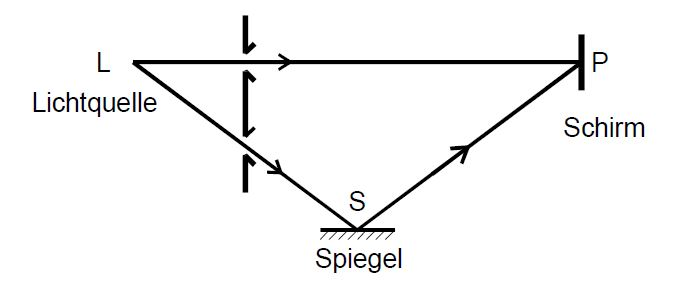
\includegraphics[height=4cm]{Unbenannt.JPG}
  \caption{Aufbau um Interferenzerscheinungen mit einer konventionellen Quelle zu erzeugen}
  \label{fig:doppel}
  \cite{skript}.
\end{figure}

Eine besondere Rolle spielt jedoch die Kohärenzlänge $l$, weshalb es nicht immer zu
Interferenzerscheinungen kommt. Da der Emissionsvorgang eine endliche Zeitspanna andauert
kann auch nur ein endlicher Wellenzug ausgesendet werden. Ist der Wegunterschied der beiden Strahlen größer
als die Länge der Wellenzüge kann es nicht zu Interferenz kommen, da die Wellenzüge zu
unterschiedlichen Zeiten im Punkt P ankommen. Die Kohärenzlänge $l$ gibt genau die Länge an, ab der
die Interferenz verschwindet.
Es gilt folgender Zusammenhang zwischen der Anzahl der beobachten Maxima $N$, der
Wellenlänge $\lambda$ und der Kohärenzlänge $l$:
\begin{equation}
  l=N\lambda
\end{equation}

\subsection{Das Michelson-Interferometer}
Beim Michelson-Interferometer wird der Lichtstrahl mit Hilfe eines semipermeablen Materials im Punkt P, dass
als Strahlteiler fungiert in zwei Strahlen aufgeteilt. Einer der Strahlen verläuft wie in
Abbildung \ref{fig:michel} zu sehen von P zu S1 und wird dort gespiegelt. Der andere Strahl läuft von
P zu S2 und wird an S2 gespiegelt. Im Punkt P treffen die Strahlen dann wieder zusammen und
werden zum Detektor D gelenkt.

\begin{figure}[H]
  \centering
  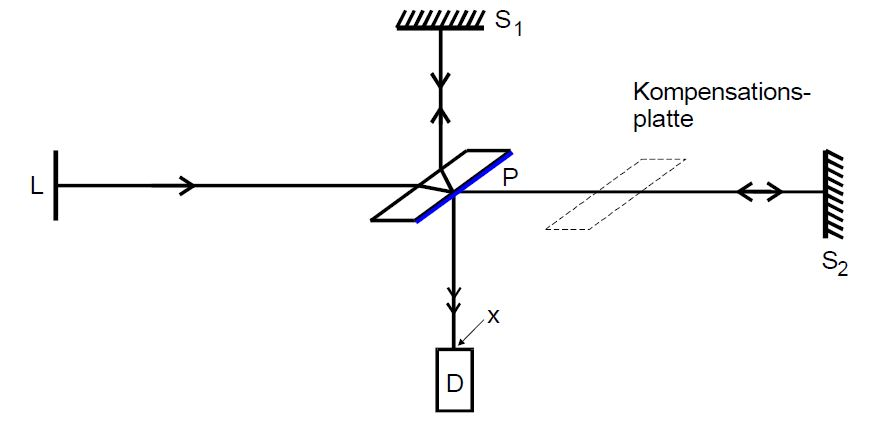
\includegraphics[height=5cm]{Michel.JPG}
  \caption{Aufbau des Michelson-Interferometers}
  \label{fig:michel}
  \cite{skript}.
\end{figure}

Auf der Strecke $\overline{PS2}$ wird eine Kompensationsplatte in den Strahlengang gestellt, diese
gleicht aus, dass der Strahl $\overline{PS1}$ das semipermeable Material dreimal durchläuft, während
der Strahl $\overline{PS2}$ dieses nur einmal durchläuft.
Sind die Strecken $\overline{PS1}$ und $\overline{PS2}$ nicht gleich kommt es zu einem Gagunterschied
zwischen den Strahlen und dadurch zur Interferenz.
Für den Fall das die Strecken $\overline{PS1}$ und $\overline{PS2}$ gleich sind beträgt der
Gangunterschied $\frac{\lambda}{2}$ und somit kommt es zu destruktiver Interferenz.
Wird  nun einer der Spiegel um $\Delta d$ verschoben, dann ändert sich das Interferenzmuster
am Ort D. Da der Zusammenhang
\begin{equation}
  \Delta d = z \frac{\lambda}{2}
  \label{interferenz}
\end{equation}
gilt, kann über diese Methode die Wellenlänge $\lambda$ des verwendeten Lasers bestimmt werden.
Mit $z$ wird die Anzahl der Maxima bezeichnet.\\

Alternativ kann der Wegunterschied über ein Medium mit anderem Brechungsindex $n+\Delta n$
verursacht werden.
\begin{figure}[H]
  \centering
  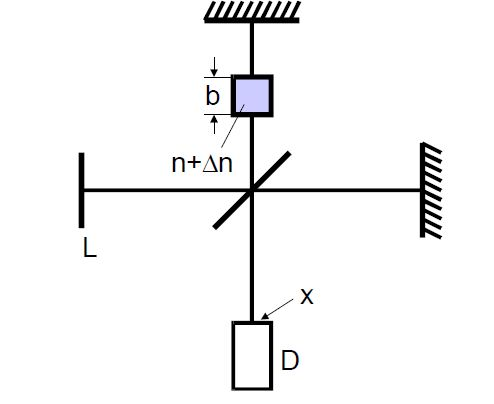
\includegraphics[height=5cm]{gas.JPG}
  \caption{Aufbau des Michelson-Interferometers mit Medium im Strahlengang}
  \label{fig:gas}
  \cite{skript}.
\end{figure}

Wenn das Medium die Länge $b$ hat beträgt der Ganunterschied $\Delta nb$.
Wird ein Gas als Medium verwendet, kann durch evakuieren oder befüllen der Zelle der
Druck $p$ variiert werden und es können die Interferenzmaxima gezählt werden.
Es gilt:
\begin{equation}
  b\Delta n = z \frac{\lambda}{2}
  \label{eqn:gas}.
\end{equation}
Für den Brechungsindex $n$ lässt sich außerdem die Formel
\begin{equation}
  n=\sqrt{1+f()\lambda)N}
\end{equation}
herleiten, wobei $N$ die Anzahl der Moleküle ist, die durch Wellen der Wellenlänge
$\lambda$ zu Schwingungen angeregt werden. Für Licht im sichtbaren Bereich lässt
sich die Formel durch die Näherung $fN<<1$  zu
\begin{equation}
  n=1+\frac{f}{2}N
\end{equation}
vereinfachen.
Außerdem wird die Annahme getroffen das sich das Gas im betrachteten Druckbereich
wie ein ideales Gas verhält. Deshalb gilt die ideale Gasgleichung

\begin{equation}
  pV=RT.
\end{equation}

Aus der idealen Gasgleichung und Formel \ref{eqn:gas} lässt sich folgende Formel für
den Brechungsindex bei Normalbedingungen $p_{0}$ und $T_{0}$ herleiten:
\begin{equation}
  n(p_{0},T_{0})= 1+ \frac{\lambda z}{2b}\frac{T}{T_{0}}\frac{p_{0}}{p-p'}.
\end{equation}
Dabei bezeichnet $T$ die Temperatur und $p-p'$ bezeichnet die Druckdifferenz in der Kammer.
Für die Brechungsindexänderung $\Delta n$ gilt außerdem
\begin{equation}
  \delta n(p,p')= \frac{f}{2}N_{L}\frac{T_{0}}{p_{0}}\frac{1}{T}(p-p')
\end{equation}
mit $N_{L}$ als Loschmidtsche Zahl.
%\cite{sample}
>>>>>>> michelson
